\scanpage{210}
\mspage{126}
% archive sheet number: 209
% element: text | top, lines 1-3 | Ceci posé
Ceci posé : \textcircled{1\textsuperscript{o}} Les six premières conditions a, a', a'', b, b', b'' sont équivalentes, \inserted{soit $P(\pi)$}, et impliquent les deux dernières
% element: diagram | upper third | P pi implies c and d
\diagram{\begin{tikzcd}[ampersand replacement=\&]
\& P(\pi)\arrow[dl,Rightarrow]\arrow[dr,Rightarrow]\&\\
c\&\&d
\end{tikzcd}}
% element: text | upper third, beneath diagram | Si pi
Si $\pi\geq\pi_1$, alors $P(\pi)$ est équivalente à \unsure{c)|c'}.
% element: deletion | middle, crossed introductory words | Les conditions
\deleted{\unsure{Les conditions}}
% element: deletion | middle, crossed block | Les conditions suivantes
\deleted{\textcircled{2\textsuperscript{o}} Les conditions suivantes sur $C,\pi_0,\pi$ sont équivalentes :

1) La condition d) implique $P(\pi)$, i.e. \unsure{on a}.}
% element: text | middle, live second assertion | Soit Filt prime
\textcircled{2\textsuperscript{o}} Soit $\mathrm{Filt}'{}^\pi\subset M$ la sous-catégorie strictement pleine de $M$ formée des objets qui satisfont la condition $P(\pi)$ ci-dessus, et $\mathrm{Filt}^\pi$ la sous-catégorie str. pleine définie dans 4.5.3 (p. 109). On a alors
% element: display | middle | Filt inclusions
\[
\mathrm{Filt}^\pi\deleted{\unsure{\subset M|\subset}}\subset\mathrm{Filt}'{}^\pi\subset M_\pi,
\tag*{(4.5.13.1)}
\]
% element: text | lower middle | et pour qu'on ait égalité
et \deleted{\unsure{on a}} \inserted{pour qu'on ait} égalité des trois membres, \deleted{pourvu que} \inserted{il suffit qu'on ait} $\pi^{\pi_0}=\pi$. Cf \inserted{prop} (4.5.6, page 116). De plus, $\mathrm{Filt}'{}^\pi$ est stable dans $M$ par $\varinjlim$ de cardinal $\leq\pi$.
% element: text | lower third, third assertion | Les conditions suivantes
\textcircled{3\textsuperscript{o}} \unsure{Les|Alors} conditions suivantes sur $C,\pi_0,\pi$ sont équivalentes
% element: text | lower third, item 3 | La condition d
\begin{enumerate}[label={},leftmargin=2em]
\item[3)] La condition d) du 1\textsuperscript{o} implique $P(\pi)$, (donc lui est équivalente), i.e. on a
% element: display | lower third | M pi inclusion
\[
M_\pi\unsure{\subset|\subseteq}\mathrm{Filt}'{}^\pi.\quad\deleted{\text{et}}
\]
% element: text | lower third, item 1 | Filt prime stable
\item[1)] $\mathrm{Filt}'{}^\pi$ est stable dans $M$ par $\varinjlim$ de cardinal $\leq\pi$.
% element: text | foot, item 1 prime | Filt prime conoyaux
\item[1')] $\mathrm{Filt}'{}^\pi$ est stable par \deleted{\unsure{lim}} conoyaux des doubles flèches.
% element: deletion | foot, before item 2 | canceled label
\deleted{\unsure{AQT|3)}}
% element: text | bottom edge, item 2 | Tout objet x
\item[2)] Tout objet $x$ de $M$ est de la forme $\varinjlim x_i$, les $x_i$ dans $\mathrm{Filt}'{}^\pi$, $I$ \unsure{grd|grand} devant $\pi$.
\end{enumerate}
% element: drawing | left of the lower list, from item 3) to item 2) | curved editorial arrow
% Its middle branch stands beside the inclusion after item 3); the lower head is beside item 2).
\figure{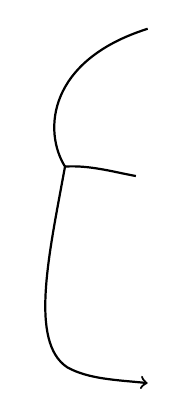
\begin{tikzpicture}[x=1cm,y=1cm]
\draw[thick,->] (1.45,4.5) .. controls (0.18,4.1) and (0.12,3.2) .. (0.40,2.75)
 .. controls (0.20,1.65) and (-0.06,0.52) .. (0.43,0.20)
 .. controls (0.70,0.05) and (1.06,0.04) .. (1.45,0);
\draw[thick] (0.40,2.75) .. controls (0.72,2.77) and (1.02,2.68) .. (1.30,2.63);
\end{tikzpicture}}
